\documentclass[11pt]{article}
%you can look for fun LaTeX packages to use hereasdf

\usepackage{amsmath}
\usepackage{amssymb}
\usepackage{fancyhdr}
\usepackage{amsthm}

\usepackage{graphicx}
\usepackage{dcolumn}
\usepackage{bm}

%fun commands for fun sets
%make sure to use these in math mode
\newcommand{\Z}{\mathbb{Z}}
\newcommand{\R}{\mathbb{R}}
\newcommand{\N}{\mathbb{N}}
\newcommand{\C}{\mathbb{C}}
\newcommand{\m}{\mathcal{M}}
\newcommand{\Tt}{\mathcal{T}}
\newcommand{\pa}{\partial}
\newcommand{\dD}{\mathcal{D}}
\newcommand{\E}{\mathbb{E}}



\oddsidemargin0cm
\topmargin-2cm    
\textwidth16.5cm   
\textheight23.5cm  

\newcommand{\question}[2] {\vspace{.25in} \hrule\vspace{0.5em}
\noindent{\bf #1: #2} \vspace{0.5em}
\hrule \vspace{.10in}}
\renewcommand{\part}[1] {\vspace{.10in} {\bf (#1)}}

\newcommand{\myname}{Alex Havrilla}
\newcommand{\myandrew}{alumhavr}
\newcommand{\myhwnum}{Hw 1}

\newtheorem{prop}{Prop}
\newtheorem{lemma}{Lemma}
\newtheorem{theorem}{Theorem}
\theoremstyle{remark}
\newtheorem*{remark}{Remark}
\newtheorem*{defi}{Def}
\newtheorem*{apps}{Application}
\newtheorem*{quest}{Question}
\newtheorem*{ans}{Answer}
\newtheorem*{interest}{Interesting}
\newtheorem*{theme}{Theme}
\newtheorem*{back}{Background}
\newtheorem*{example}{Example}

\setlength{\parindent}{0pt}
\setlength{\parskip}{5pt plus 1pt}
 
\pagestyle{fancyplain}
\lhead{\fancyplain{}{\textbf{HW\myhwnum}}}      % Note the different brackets!
\rhead{\fancyplain{}{\myname\\ \myandrew}}
\chead{\fancyplain{}{\mycourse}}

\title{2/8 Update}

\linespread{1.3}

\begin{document}



\maketitle

Note: we use x as the variable for densities and y as the variable for characteristics.

\section{Lower Bounds for Small p}

I verified the density for $X^{(b)}_p = X^{(b)}/||X^{(b)}||_p$ where $X^{(b)} \sim (1-b+bx^2)e^{-x^2/2}$ is convex. See:

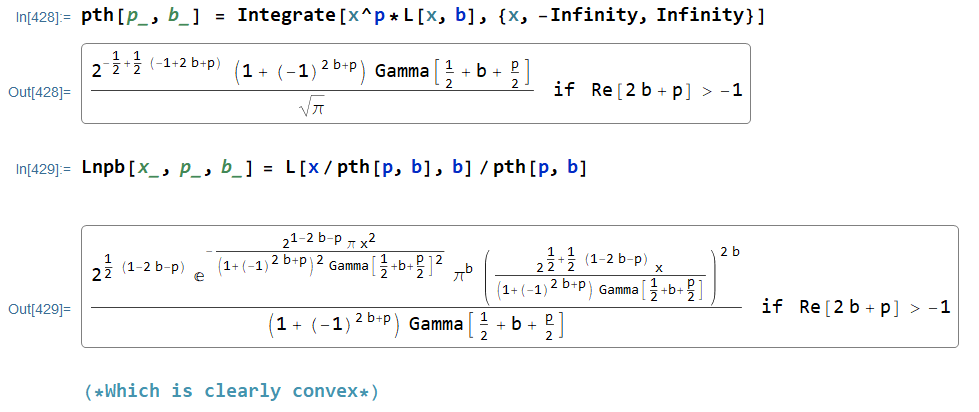
\includegraphics[width=500px]{C:/Users/Alex/Desktop/Notes/TkoczResearch/pics/small_p_convexity.png}

Note the density is a gaussian times a monomial which is convex in $y$ for arbitray $b$ and thus the difference  $f_b-f_0$ will have two zeroes.


\section{Higher Order Atoms}

Let 

\begin{align*}
	L_n(x) = x^{2n} e^{-x^2/2}
\end{align*}

to verify this is a type L density we compute the FT and note all the zeroes are real and symmetric. So we compute

\begin{align*}
	I_n = \int_{\R} x^n e^{-x^2/2}e^{-iyx}dx
\end{align*}

We note via differentiation in y and DCT we have the reccurence relation $I_{n+1}(y) = iI_n'(y)$. So in particular $I_{2n+2} = - I_{2n}''$. This, in addition to the initial condition $I_0(y) = e^{-y^2/2}$, gives

\begin{align*}
	I_{2n} = (-1)^n \frac{d}{dy}e^{-y^2/2} = (-1)^ne^{-y^2/2}H_{2n}
\end{align*}

where $H_{2n}$ denotes the 2nth hermite polynomial. It is well known these polynomials have all real zeroes(via Gauss-Lucas) and further $H_{2n}$ is an even function($H_{2n+1}$ is odd). Thus we conclude $L_n$ constitutes a valid type L density.

\begin{remark}
	Perhaps there is something interesting to be done using the fact these characteristic functions are the hermite polynomials. Not sure.
\end{remark}

\textit{Some Philosophy:} I hoped to go on establishing khintchine type inequalities for these RVs and extend "atomic structure" we started with the $n=1$ case. But the convexity technqiue we used to show the inequalities for $n=1$ seeems to require more work. Consider a plot of the second derivative of the density:

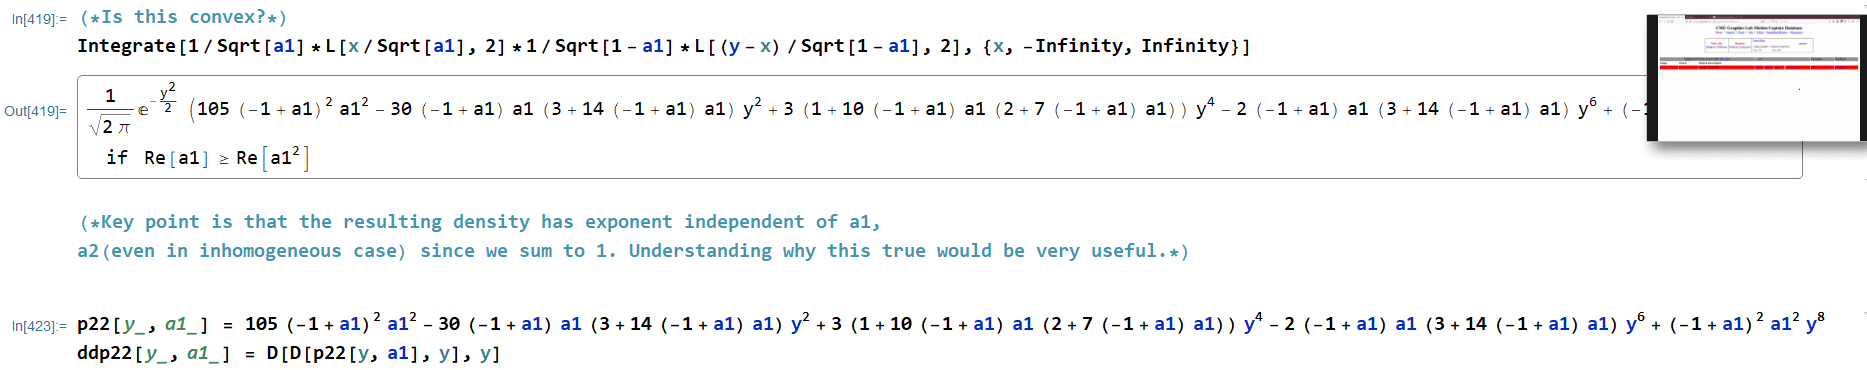
\includegraphics[width=500px]{C:/Users/Alex/Desktop/Notes/TkoczResearch/pics/high_atom_non_convexity1.png}

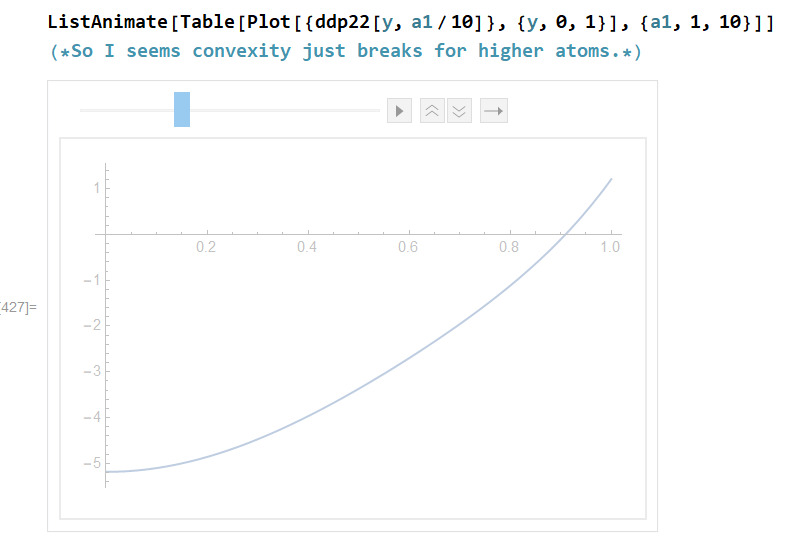
\includegraphics[width=500px]{C:/Users/Alex/Desktop/Notes/TkoczResearch/pics/high_atom_non_convexity2.png}

Ie. the function is not convex. Yet there do seem to be 2 zeroes when we look at an $\epsilon$ difference:

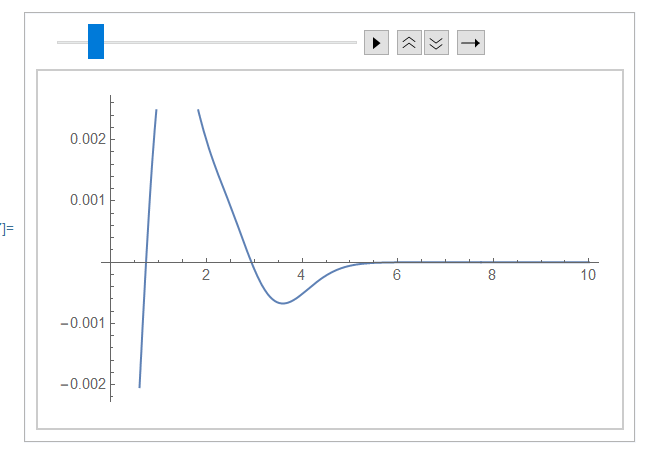
\includegraphics[width=500px]{C:/Users/Alex/Desktop/Notes/TkoczResearch/pics/high_atom_2_zeroes.png}

So we could still hope to recover khintchine inequalities here using the technique. But some more work is required.

\begin{quest}
	A key point in all these computations is that the dependence on $a_1,a_2$ disappears. After putting some work into doing the computation
	\begin{align*}
		\int_{\R} x^{2n}e^{-x^2/2a_1^2}x^{2m}e^{(y-x)^2/2a_2^2}dx
	\end{align*}

	I am still not sure why. Understanding would help greatly in this general case(mathematica fails here).
\end{quest}

\begin{ans}
	Look at it on characteristic side and take inverse fourier transform.
\end{ans}


\end{document}

